\chapter{VxWorks代码插入方案分析与设计}

VxWorks操作系统是美国风河公司旗下的一款嵌入式实时操作系统。
该系统由于其高实时性、高可靠性,在嵌入式实时操作系统领域
占据一席之地,特别是应用于通信、军事、航空航天等
高精尖领域中。

VxWorks 5.5是VxWorks系统中一个较为经典的版本。
本课题的所有研究都围绕VxWorks 5.5来展开,
后文如果没有特别说明,
所有的VxWorks都是指5.5版本。

VxWorks作为嵌入式操作系统,
与PC系统有很大的不同之处。
体现在系统的加载启动流程,与硬件的交互等多个方面。
虽然VxWorks也使用了ELF文件格式作为它的
可执行文件格式,并且也是用gcc编译器。
但是正如\ref{twoqs}中所述,
代码插入决不只是针对ELF文件格式和内容的修改,
还与系统的内存空间等有着密切的联系。

本章在前文列举的所有针对ELF代码插入技术的基础上,
加上针对VxWorks若干特性的分析,
考察这些代码插入技术在VxWorks中应用的可能性,
并选择合适的代码插入方案。

%%%%%%%%%%%%%%%%%%%
%%%%%%  3.1  %%%%%%
%%%%%%%%%%%%%%%%%%%

\section{VxWorks镜像文件格式}

VxWorks的系统镜像文件本身就是一个ELF静态链接可执行文件,
因此我们在前文中对ELF格式等方面的讨论在这里同样适用。
为了寻找能够插入代码的位置,
我们需要考察系统镜像文件的节头表和程序头表。
图\ref{shtandpht}展示了映像文件的
节头表和程序头表,以及他们的映射关系。

\begin{figure}[h!]
    \centering
    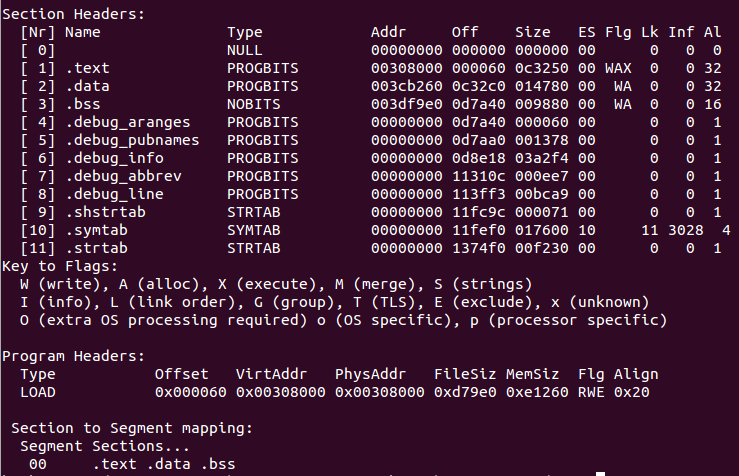
\includegraphics[width=0.68\textwidth]{figure/shtandpht.png}
    \caption{VxWorks系统映像文件的节头表和程序头表}
    \label{shtandpht}
\end{figure}

该ELF文件的布局不同于一般的Linux下的ELF文件。
Linux下的ELF文件一般有两个加载段,
一个只包含代码,拥有可读和可执行的权限;
一个只包含数据,拥有可读和可写的权限。

而VxWorks系统镜像文件的布局要更加简单,
只有一个可加载段,对应三个节,
分别是text节,data节和bss节。
一般来说,ELF文件中的代码和数据由于分别具有不同的属性
(例如代码节不可写,数据节不可执行),
这两种节会被映射到不同的段来映射,
从而映射到不同的页面,
并在页表中赋予他们不同的属性。
然而VxWorks的做法比较特殊,
代码和数据节映射到一个段,
这也就意味着该段必须同时具有可读可写和可执行三类属性。

然而,由于VxWorks系统镜像文件只有一个段,
也就导致我们无法利用段与段之间由于
地址对齐而产生的地址空间。
因此,我们在寻找空闲地址空间的过程中,
可以利用两类办法:

1、利用.text节之前或者.bss节之后的地址空间

2、利用该加载段中的nop指令串



%%%%%%%%%%%%%%%%%%%
%%%%%%  3.2  %%%%%%
%%%%%%%%%%%%%%%%%%%

\section{VxWorks运行时内存布局}
\label{neicunbuju}

回顾在\ref{twoqs}中提到的关于ELF文件插入的两个问题:
文件空间与地址空间。
要寻找合适的空闲的地址空间,
我们需要熟悉VxWorks运行中的详细内存布局。

图\ref{ram}是在x86硬件平台下的VxWorsk内存布局的一个简略版本。

\begin{figure}[h!]
    \centering
    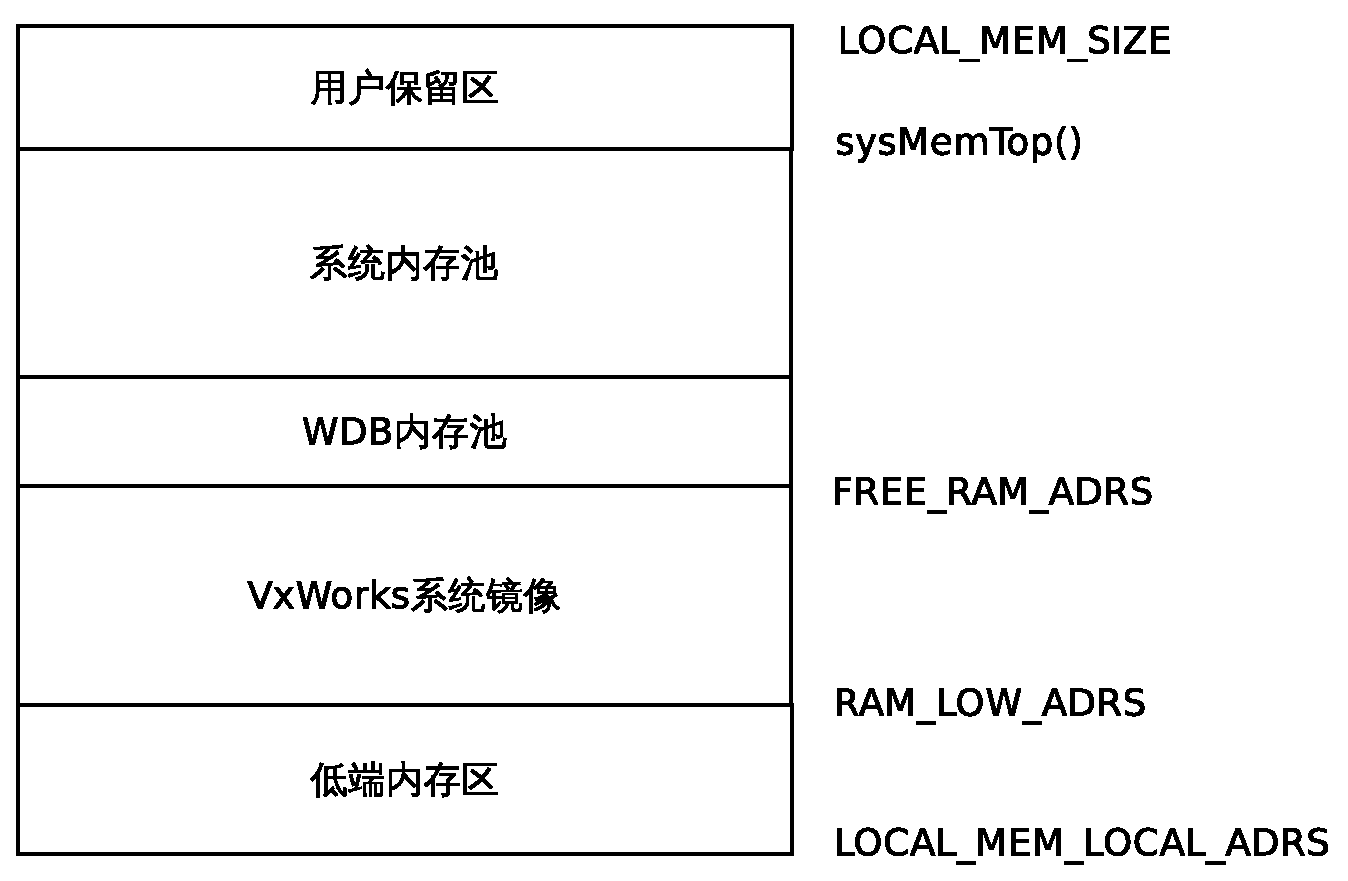
\includegraphics[width=0.68\textwidth]{figure/ram.eps}
    \caption{x86下的VxWorks系统内存布局}
    \label{ram}
\end{figure}

我们的目标是寻找空闲的地址空间,
使得代码能够映射到这一块地址并被执行。
然而,从图中不难看出:
在VxWorks系统镜像的低地址和高地址两个方向,
均有明确的定义和用途。
其中,RAM\_LOW\_ADRS之前的低端内存区,
被用作初始化堆栈。
系统的初始化流程借助这一区域实现函数调用。
而FREE\_RAM\_ADRS之后的地址,
用于WDB内存池。
这两段地址皆有明确的用途。
这也就意味着,我们在上一节中提到的
第一类方法,即利用.text节之前或者.bss节之后的地址空间
进行插入的办法可能无法使用。
然而利用nop串进行插入仍然是可行的办法之一。


%%%%%%%%%%%%%%%%%%%
%%%%%%  3.3  %%%%%%
%%%%%%%%%%%%%%%%%%%

\section{VxWorks代码插入方案设计}

\subsection{利用nop指令串插入}

在\ref{nopinjection}中我们曾指出,
由于体积较大,VxWorks系统镜像中存在较多的nop
指令串可以用于插入代码。

然而手动进行插入少量代码方式虽然简单,
但若对较大的文件注入大量的代码,
手工操作的工作量会很大。
\cite{infelf}提供的infelf工具,
可以用于在Linux下的ELF文件中自动寻找所有的
nop指令串。我们在其基础上,
完善了一个代码插入工具。
该工具可以自动寻找VxWorks
系统镜像中所有可以用于插入的
nop指令串。该工具还可以以一个包含汇编代码的文本文件为输入,
自动将代码汇编为二进制机器代码后,
插入到nop指令串中。

该工具的完整C语言代码参见附录\ref{python},
工具的输入为VxWorks镜像文件和待插入的汇编代码文件。
工具的主要算法如下:

1、反汇编VxWorks文件,找到所有的ret指令。

2、对于所有的ret指令之后的第一条指令,如果为nop,则标记为nop-start。

3、对于所有的nop-start之后的指令,第一条地址为16的倍数的指令,将其标记为nop-end。

4、将输入的汇编代码文件汇编为二进制代码,从第一个nop-start处开始插入。

5、每插入一条指令,检测到nop-end的距离,如果小于jmp的长度或者下一条待插入指令的长度,则将上一条指令修改为jmp,
目的地址为下一个nop-start。直到二进制代码插入完成。



\subsection{通过扩展.bss节进行插入}

前文中已经指出,.bss节之后的地址用于WDB内存池,
因此无法用于插入二进制代码。
然而,我们可以通过修改BSP的办法,
重新生成bootloader。
修改bootloader的目的是让它在加载镜像文件的过程中,
为我们预留.bss之后的一段地址。
即把WDB内存池的起始地址略微后移,
从而留出空闲的地址空间用于插入。

BSP是Board Support Package(板级支持包)的缩写,
是Wind River公司推出的针对不同的硬件平台的一个程序。
该程序针对不同的硬件进行抽象,
为上层的VxWorks操作系统提供一致的接口,
从而屏蔽了底层硬件的诸多细节,例如内存布局等等,
在一定程度上方便了VxWorks驱动程序和应用程序的开发。
BSP和VxWorks的关系如图\ref{bsp}所示。


\begin{figure}[h!]
    \centering
    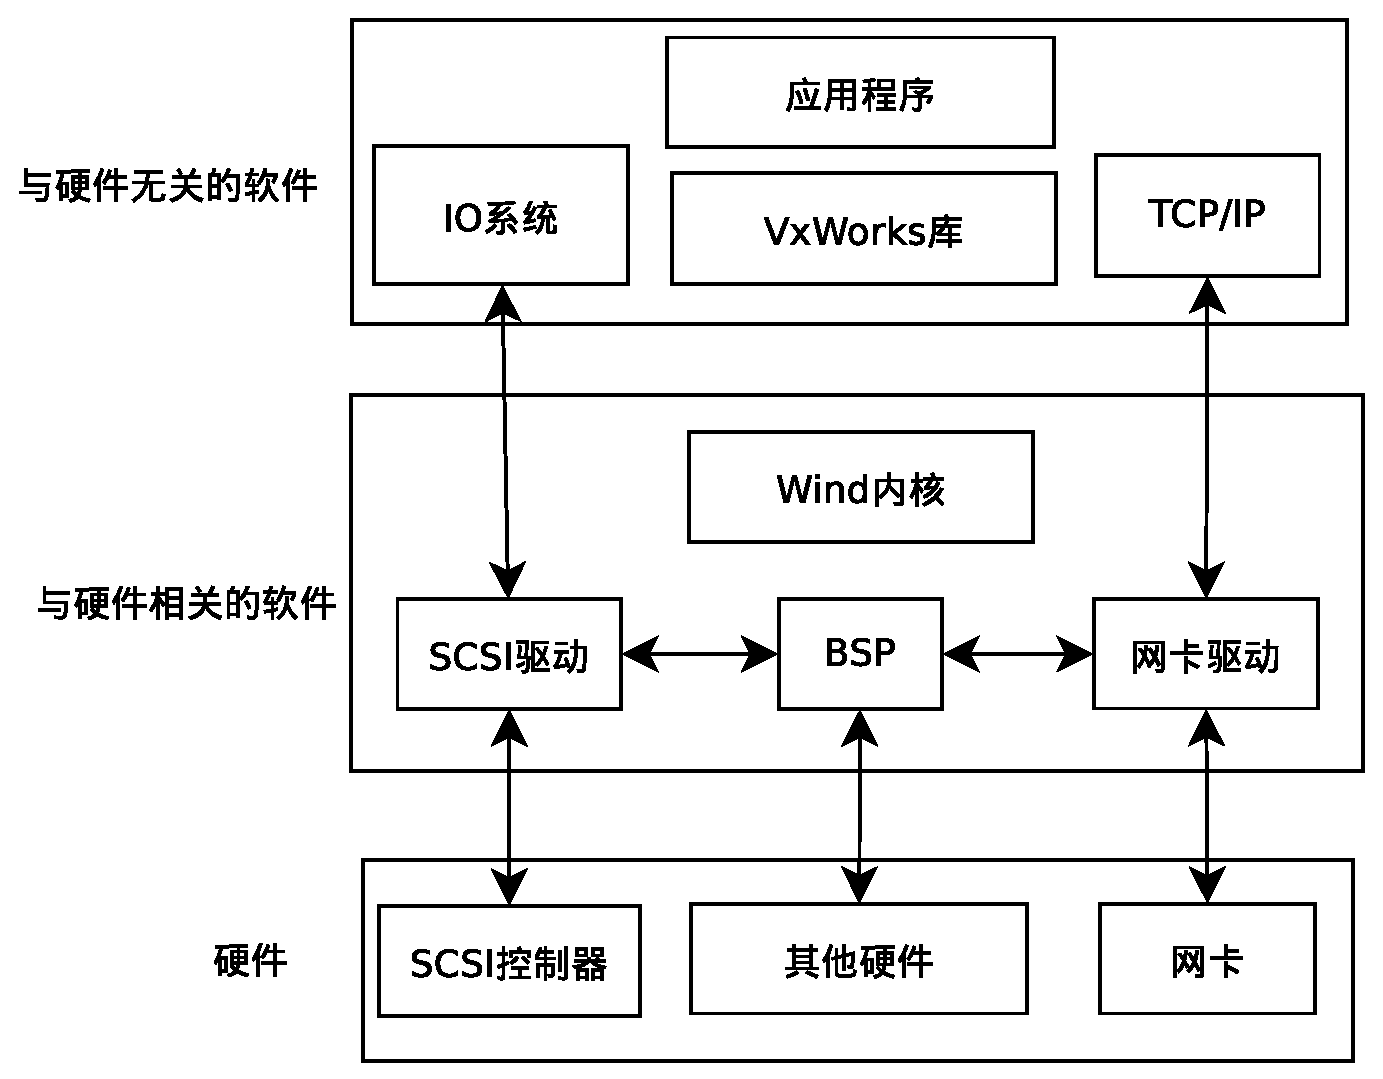
\includegraphics[width=0.63\textwidth]{figure/bsp.eps}
    \caption{BSP与VxWorks操作系统的关系}
    \label{bsp}
\end{figure}


可见,BSP直接或者间接地与硬件进行交互,
并为上层的软件提供接口。
BSP对硬件的一个比较重要的抽象就是内存布局,
\ref{neicunbuju}中的图\ref{ram}所描述的VxWorks内存布局,
包括各个重要地址的位置,其实都是在BSP文件中定义的。

为了达到我们目标,即使得代码可以插入在.bss节之后
并不影响系统的正常运行。
我们只需要修改BSP中的宏FREE\_RAM\_ADDRESS即可。
例如,我们将该字段增大0x1000。
修改后,VxWorks的内存布局将会如果\ref{ram2}所示。

\begin{figure}[h!]
    \centering
    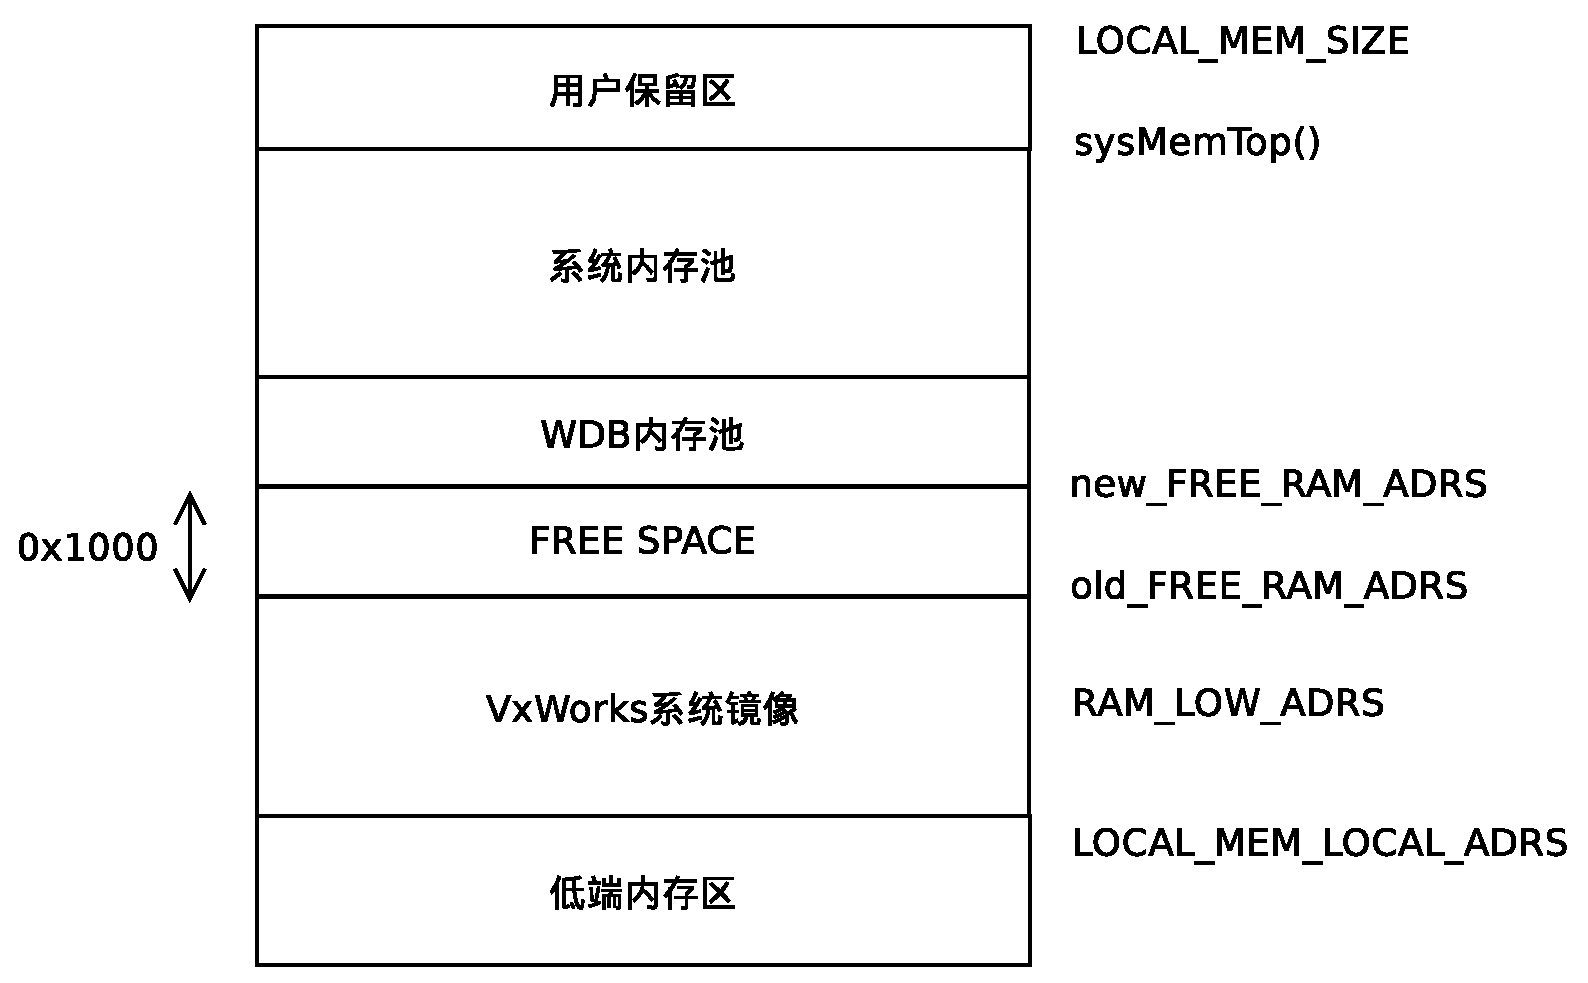
\includegraphics[width=0.75\textwidth]{figure/ram2.eps}
    \caption{修改BSP后的VxWorks系统内存布局}
    \label{ram2}
\end{figure}

这样,我们就有了一定的内存空间用于插入代码。
这时我们就可以使用附录\ref{python}的插入工具
对VxWorks镜像进行代码插入了。

这里的插入算法与\ref{after}中有些许不同,具体的插入算法如下所示。

1、找到第一个(也是唯一一个)加载段的位置,
将该段的filez字段和memsz字段增加要插入代码的大小。

2、将.bss节的len字段增加插入代码长度大小。

3、对于在代码段之后的所有节区,将其offset字段增加一页(4KB)的大小。

4、将插入代码的长度填充到1页(4KB),然后插入到原.bss节最后的位置。

























